\chapter{绪论}
\section{研究背景及意义}
随着信息通信技术的快速发展,无线感知系统与传统通信网络的整合成为了研究的重要方向。
《物联网新型基础设施建设三年行动计划(2021-2023年)》明确指出,物联网是通过感知技术和网络通信技术实现人、机、物的泛在连接,
为社会经济的数字化转型和智能升级提供了重要的基础设施支持\cite{IoTActionPlan2021}​​。这个行动计划突显了感知技术在现代通信网络中的核心地位。
另外,从《十四五”信息通信行业发展规划》中我们可以看到,
我国在信息通信领域的总体发展战略中,也明确了建设融感知、传输、存储、计算、处理为一体的新一代通信网络基础设施,
实现感知技术和通信技术的融合发展,强调了信息通信行业面向新阶段高质量发展的重要性\cite{14thFiveYearPlan}​​。

基于Wi-Fi,蓝牙,毫米波,调频载波(Frequency Modulated Continuous Wave,  FMCW)等无线通讯技术的的室内被动定位以及人体监测技术在前些年得到了飞快的发展,
基于这些技术人们开发了被动室内定位,婴幼儿监测,老人跌倒监测,非入侵的生理信息获取,姿势识别以及人员识别等应用。
然而这些技术在成本、精度等方面始终难以满足要求,本研究着重于探索UWB技术在室内被动定位以及人体监测方面的潜力。

UWB技术始于20世纪60年代兴起的脉冲通信技术。UWB技术利用频谱极宽的超宽基带脉冲进行通信,过去主要用于军用雷达、定位和低截获率/低侦测率的通信系统中\cite{uwb_history}。
由于UWB技术具有数据传输速率高(达1Gbit/s)、抗多径干扰能力强、功耗低、成本低、穿透能力强、截获率低、与现有其他无线通信系统共享频谱等特点\cite{uwb_survey},
成为无线个人局域网通信技术的首选技术。

过去UWB主要应用于军事领域,近些年来,随着UWB芯片的商品化以及成本下降,
Time Domain、Ubisense、Bespoon以及Qorvo等公司开始提供用于定位的UWB芯片,国内诸如清研讯科,沃旭通讯和易百徳等公司也开始研发国产替代。
在智能汽车领域,宝马iX M60和iX xDrive40, 蔚来ET7等车型已经率先开始搭载UWB数字钥匙,特斯拉、大众、奥迪、长城、奇瑞等车厂也都对UWB技术开始布局。
在智能手机领域,苹果率先在iphone11上搭载自研的超宽带U1芯片,三星以及小米等厂商也纷纷跟进\cite{uwb_cellphone}。
在智能家具方面,苹果的HomePad,AirTag,三星的Galaxy SmartTag等产品也开始搭载UWB芯片,小米手机通过UWB一指连,可以对部署了UWB芯片的小米电视、音箱、电风扇、台灯、笔记本等众多智能产品实现操控。

过去的UWB被动感知研究需要用到昂贵的矢网,或者需要设备间有接近完美的时间同步,以及较高的采样率,这些因素限制了UWB被动感知的应用。
得益于UWB的广泛部署,基于UWB信道脉冲响应的环境感知技术在过去几年开始受到关注,研究人员在利用UWB信道脉冲响应进行室内定位、人体监测等领域取得了初步的成果,
这些工作基于已有的UWB硬件,无附加成本,易于部署,
但是系统的性能与现有的基于Wi-Fi或是毫米波的系统仍然有较大差距,具有较大的提升空间。本文着重于探索UWB芯片在通讯之外的感知能力。


\section{国内外研究现状}

\subsection{被动室内定位技术}
被动室内定位系统是指被定位目标无需携带任何硬件,人员可以不携带任何电子设备,无线感知系统通过分析人员对环境中电子信号的影响得出人员的位置。
UWB CIR是传输链路的时域信息,它表达了链路上不同传输时间的传输路径产生的信号强度。
UWB CIR的变化对应环境的变化,通过研究CIR的变化可以得到环境变化的信息。
基于UWB CIR的室内定位系统主要依靠CIR的变化得出运动目标的飞行时间(time of flight, TOF),通过TOF进行定位。

Ledergerber等人\cite{Ledergerber}首先提出使用低成本超宽带设备 dwm1000 进行无设备的行人追踪问题。
作者指出,许多设备,如汽车钥匙、手机和WiFi路由器,都配备了UWB芯片。
这些设备经常估计信道脉冲响应来解码传输的数据或估计飞行时间进行定位。
本研究详细调查了如何利用这些CIR测量来增强超宽带通信和定位网络,将其转化为一个多静态雷达网络。
通过使用现成的硬件采集,过滤,分析CIR数据,
通过计算累积方差并进行背景减除提取运动物体的信号特征,通过在方差上运行滑动窗口算法定位目标位置,通过粒子滤波在空间中采样,
做到了实时跟踪在配备超宽带模块的空间内行走的无标签人员。
这种技术为智能家居应用,如智能音响、老年人监控和安全系统,提供了新的可能性。

Bocus等人\cite{Bocus2021}使用Ledergerber等人采集的数据集,改进了特征提取算法,进一步提升了系统的性能。
与Anton相同,首先也是对累积方差进行背景减除来移除雷达数据中的静态元素。
为了减少雷达中的静态杂波并增强连续扫描中的变化,作者添加了特定的差分滤波器作为运动检测滤波器。
这有助于突出由移动目标引起的变化。
作者还沿着快时间轴应用了带通滤波器,以消除发射机和接收机之间的噪声和串扰信号。
为了进一步清洗数据并拒绝杂波,作者使用了RPCA(Robust Principal Component Analysis, 鲁棒主成分分析技术)。
RPCA是一种矩阵分解技术,它将输入矩阵(在这种情况下是雷达扫描数据矩阵)分解为两个矩阵的总和:
一个低秩矩阵和一个稀疏矩阵。这种分解有助于强调目标的信号,同时抑制背景噪声和杂波。

Li\cite{VATS}等人也使用Ledergerber等人采集的数据集。
作者提出了一种基于方差的时空映射算法(VATS, variance-based temporary-spatial),
该算法把方差值映射到二维空间中的椭圆上,做为行人处于该椭圆的概率。
并且从最大后验概率的角度解释了缓解干扰的原理。
实验结果表明,所提出的VATS映射算法实现了50th和90th百分位误差分别为0.156m和0.272m,
这对于实际应用来说是有希望的。

FMCW(Frequency Modulated Continuous Wave, 频率调制连续波)雷达发送频率调制的信号,
通过接收信号的频率差得到发射物体的TOF,也在TOF的基础上进行定位,
相比UWB雷达,FMCW雷达可以达到更高的采样频率与精度,
但是需要特定的硬件,相应的系统成本更加昂贵。
Fadel等人\cite{Adib_tracking,Adib2015MultiPersonLV}采用了多位移FMCW技术,
构建了一个基于FMCW的室内定位系统(WiTrack2.0),该系统能够追踪用户的动作,而无需用户携带或佩戴任何设备。
该系统通过共享频带实现多雷达协同工作,通过消去背景信号得到单个运动目标的定位,
在此基础上通过多个雷达融合定位实现了对于多个运动目标的定位,
通过多分辨率分析感知由于呼吸而引起的微小运动来提取静态目标的信息。
实验结果显示,该系统可以同时定位多达五个人,每个x/y维度的中位数精度为11.7 cm。

Wi-Fi的信道状态信息(Channel State Information,CSI)对应CIR的频域信息,
也可以用来对运动目标进行定位。相比于超宽带,Wi-Fi采用了MIMO与OFDM技术,可以同时得到多个载波的信道信息。
Qian等人\cite{Qian}提出了Widar系统,通过Wi-Fi的CSI信息得到运动目标的多普勒频移,
建立多普勒频移与运动目标位置的模型,从而得到位置,实现了0.35m的定位精度。
但是Widar需要需要多条通讯链路从而得到目标的位置。
Widar2.0使用单个Wi-Fi接入点实现了0.75m的定位精度,该系统探索CSI与TOF,AOA,
以及多普勒频移的关系,从而得到运动目标的位置。

\subsection{人体活动检测技术}
被动人体活动检测系统不需要检测对象携带任何设备,无线感知系统通过检测信号覆盖范围内人体活动造成的扰动,从而进一步对人体的动作、手势等运动进行识别。
被动人体活动检测主要通过视觉,超宽带,Wi-Fi以及毫米波雷达实现。

Wi-Fi的信道信息(Channel State Information, CSI)在近年来已经被广泛研究,用于搭建被动人体活动识别系统。
这些系统的理论依据是,由于人体70\%由水组成,因此它可以反射Wi-Fi信号。因此,通过监测Wi-Fi信号的变化,可以识别人体活动。
Wang等人\cite{WiFi_Wang_HAR}提出了一个基于Wi-Fi CSI的无设备人体活动识别系统CARM。CARM的独特之处在于它基于两个理论模型:
首先,他们提出了一个CSI-speed模型,量化了CSI动态和人体运动速度之间的关系。
其次,他们提出了一个CSI-activity模型,量化了人体运动速度与人体活动之间的关系。
基于这两个模型,他们在商用Wi-Fi设备上实施了CARM。实验结果显示,CARM达到了96\%的人体活动识别率,并且对环境变化具有很强的鲁棒性。

UWB CIR对应信道状态信息的时域表示,也可以用来表达传输链路的物理层信息,
Bocus等人\cite{Bocus_comp}的研究对比了超宽带CIR与Wi-Fi CSI信息用于人体活动监测的分析的可行性,
研究发现超宽带的信号分辨率更高,噪声更小,相比于Wi-Fi在人体活动检测方面应该能取得更好的成果。
与此同时,他们还发布了两个数据集,一个是基于UWB CIR的定位与HAR数据集\cite{Bocus_dataset},
另一个是基于UWB、WiFi CSI的多模态多人定位与HAR数据集\cite{Bocus_dataset_IPL},为后续使用UWB CIR实现多人定位与HAR提供了便利。

与传统的人体活动识别系统相比,如使用摄像机、雷达或可穿戴设备的系统,基于Wi-Fi和UWB信号的系统具有多种优势。
它们不需要额外的设备,仅通过人体反射的无线信号检测活动。
此外,Wi-Fi和UWB信号可以穿透墙壁、家具和门,而摄像机则需要良好的照明条件。 

Wang等人\cite{Wang_Wifi_HAR}提出了一个名为“m-Activity”的系统,
专为通过商用毫米波雷达进行人体活动识别而设计。
该系统有效地减少了由环境多径效应引起的噪声,
从而从嘈杂的背景环境中提取出与人体活动相关的关键信息。
为了进一步提高识别的准确性,Wang等人设计了一个轻量级的神经网络HARnet,
专门用于对处理后的毫米波雷达点云进行推断。
此外,为了满足实时应用的需求,他们还引入了一个高效的响应机制,
确保系统能够在短时间内给出识别结果。经过多次实验验证,
该系统在3米的检测范围内,对五种预定义的人体活动实现了93.25\%的离线准确率和91.25\%的实时准确率。
更为重要的是,无论是在简单还是复杂的环境中,该系统都表现出了对多径效应的良好适应性,
证明了其在实际应用中的潜在价值。

利用视觉信息进行人体活动检测的设备具有代表性的是英特尔公司的深度摄像机RealSense D455以及微软公司推出的Kinect,
深度摄像机含有RGB摄像头、红外检测仪,可以检测物体的深度信息,利用视觉以及深度信息实时进行手势识别以及骨骼检测。

\subsection{生理信号检测技术}
Heba等人\cite{UbiBreathe}开发了基于Wi-Fi接收信号强度的UbiBreathe系统,
使用常用的Wi-Fi设备,利用接收信号强度(receiced signal strength,rss)
的变化来实现呼吸监测,只需被监测对象站在发射装置与接收装置之间,
该系统可以无创地估计呼吸率并检测呼吸暂停,
对呼吸暂停检测的准确性超过96\%,
对呼吸率的估计误差小于每分钟一次呼吸,
为呼吸监测提供了一个非侵入且高度准确的解决方案。

Fadel等人\cite{Adib_Breathe}基于FMCW雷达,开发了一套被动呼吸监测系统,该系统利用调频载波的相位变换采集人体呼吸时胸腔的微小运动信息,
通过解析人体对应时间点的相位变化得到对于人体呼吸的估计,该系统在滤除呼吸信号后,还可以实现对心跳信号的监测。
基于FMCW技术开发的毫米波雷达也被广泛应用于呼吸监测,Zhao等人\cite{zhao_Breathe}用单个毫米波雷达实现了多目标无接触呼吸心跳监测,心跳监测的误差达到了7.77\%。

超宽带雷达具有GHz级别的频率,与FMCW雷达一样,它的波长也是cm级别的,所以它的相位变化应该也能够很好的反应出呼吸时胸腔的运动,目前尚无相关文献对这一可能性进行尝试。

\section{本文主要工作与结构安排}
\begin{figure}[htbp]
    \centering
    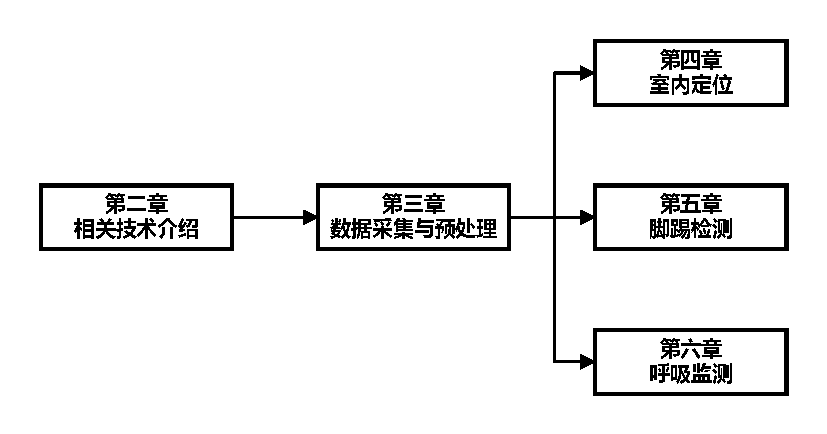
\includegraphics[width=.7\linewidth]{imported/本文章节内容组织架构图}
    \caption{\label{fig:structure}本文章节内容组织架构图}
\end{figure}
本文共有七个章节,各章节围绕 UWB信道脉冲响应 被动感知算法 所涉及的背景知识、
数据采集与预处理方法、粗粒度的被动定位算法、中粒度的脚踢检测算法,以及细粒度的呼吸监测算法展开,组织结构图如图\ref{fig:structure}所示:

第一章介绍了本文研究背景及国内外研究现状,针对当前基于通讯信号的被动感知技术的研究现状进行了总结,
介绍了国内外在被动室内定位,人体活动检测以及生理信号监测方面的研究现状。
提出当前基于UWB信道脉冲响应的被动感知算法发展不完善,未能发掘UWB信号噪声小,精度高的优势,需要在不同粒度上探索UWB信道脉冲响应的被动感知能力。
最后总结了本文的章节结构。

第二章主要介绍本文涉及的UWB技术以及其信道脉冲响应的特征、
被动感知算法中涉及的深度学习、粒子滤波、聚类等相关理论与技术。
整体架构、预测性维护的相关理论与技术。

第三章描述了对UWB CIR信号的采集与预处理步骤,提出通过上采样以及匹配滤波提高信号的分辨率,
利用UWB CIR信号相对稳定的特征,通过correlation匹配时延与相位,通过累积平均以及背景滤除来初步提取信号中的特征。
第三章为后续的四、五、六章节提供了数据基础。

第四章描述了基于UWB CIR的被动室内定位算法,提出了通过神经网络替代传统的滑动窗口算法提取信号中的空间特征从而找到人的位置,
利用粒子滤波提取数据的时空特征从而实现追踪,最后把粒子送入聚类算法找到人的位置。

第五章描述了基于UWB CIR的脚踢检测算法,通过CNN+LSTM网络提取信号中的时空特征,在实验室和实车上实现了脚踢检测算法,
可以用于替代传统的电容检测方案,精度更高,且不需要额外的硬件。

第六章描述了基于UWB CIR的呼吸监测算法,通过傅里叶变换和带通滤波器提取CIR信号相位的频域特征,找到人的位置及其呼吸信号,
进一步探索信道脉冲响应的相位在细粒度感知上的潜力。

第七章总结了本文所做的关于UWB CIR被动感知方面的研究工作,并提出对其未来研究方向的规划。
\chapter{相关技术}
\section{引言}
\section{UWB CIR相关技术}
\subsection{UWB的定义}
UWB技术是一种短程无线通信协议,它使用从3.1到10.5 GHz的频率范围的短脉冲的无线电波,
UWB技术可以使用非常低的功耗进行短程、高带宽通信,覆盖了大部分无线电频谱。
UWB的带宽通常有两种定义,一种定义要求带宽大于中心频率的20\%,如\ref{eq:UWB_bandwidth_def_1}所示:
\begin{equation}\label{eq:UWB_bandwidth_def_1}
    B_f=\frac{2\left(f_H-f_L\right)}{f_H+f_L} \geq 0.2
\end{equation}
另一种定义要求带宽大于500MHz,如\ref{eq:UWB_bandwidth_def_2}所示:
\begin{equation}\label{eq:UWB_bandwidth_def_2}
    f_H-f_L \geq 500 \mathrm{MHz}
\end{equation}
这里\(f_H\) 和 \(f_L\)是指上限频率和下限频率,通常定义为相对于主峰小10dB的频率\cite{UWB_Characteristics}。

\subsection{UWB的特点}

\subsubsection{信道容量大}
在加性高斯白噪声信道中,信道的理论无错容量可以从香农公式\cite{Shannon}计算出来。香农公式如\ref{eq:Shannon}所示:
\begin{equation}\label{eq:Shannon}
C=B \log _2\left(1+\frac{\int_B P_d(f) \mathrm{d} f}{\int_B N_0 \mathrm{~d} f}\right)
\end{equation}
其中C是信道容量(bit/s),B是信道带宽(Hz),\(P_d(f)\)是信号功率谱密度(dBm/Hz),\(N_0\)是噪声功率谱密度(dBm/Hz)。

UWB设备的信道带宽往往大于500MHz,远远大于Wi-Fi,蓝牙等技术。更大的带宽使得UWB可以同时在多个频段上传递信息,
香农公式也指出了信道容量与信道带宽成正比,所以UWB拥有远大于一般通讯协议的信道容量。
目前搭载了UWB芯片的智能设备之间的数据传输速率往往能达到480 Mbps 到 2 Gbps。

\subsubsection{功耗低}
因为 UWB 信号占用了超过500MHz的带宽,根据香农公式,在相同的噪声水平下,要达到相同的通讯速率,带宽越大,功耗越小。
同时UWB的单次脉冲通常实在纳秒级别,信号持续时间短,系统大多数时间处于休眠状态,更进一步降低了功耗。
UWB的通讯功耗在几百微瓦到几十毫瓦之间,远远小于CDMA,蓝牙等技术,有助于延长设备的续航时间\cite{CDMA}。

\subsubsection{截获率低}
如上所述,UWB带宽大,功耗低,且可以以每秒数百万比特的独特随机化时序码进行通信,
每个比特通常由非常低幅度的大量脉冲表示,通常低于噪声水平,基本上可以被当作是噪声。
这些特性使得UWB具有很好的隐蔽性和很低的被截获概率。

\subsubsection{共享频谱}
正是因为UWB设备功耗低,信号幅度通常低于噪声水平,对其它窄带无线通讯协议的干扰非常小,从而使得UWB设备可以与其它无线通讯协议共享频谱,提高了频谱利用率。

\subsubsection{抗多径干扰能力强}
相比与窄带信号,UWB信号的频谱更宽,对应在时域上信号更窄,UWB在时域上的脉宽是纳秒级别的。
脉冲信号相互重叠时,多径难以分辨,而UWB信号经过不同路径到达接收端的信号重合的概率低,给了UWB协议很好的多径分辨率,
这有助于实现高精度定位,同时也有助于提高信道脉冲响应对环境的感知能力\cite{xhl_thesis}。

\subsection{CIR的定义}
信道脉冲响应提供了关于电磁波在空间中传播的信息。
在UWB通讯系统中,发送设备和接收设备会计算它们之间的信道脉冲响应,
信道脉冲响应的可以表示为\ref{eq:CIR}:
\begin{equation}\label{eq:CIR}
    h(t)=\sum_{p=0}^{P-1} \alpha_p \delta\left(t-\tau_p\right)
\end{equation}
其中,\( P \) 是多径信道中的路径数量,
\( \alpha_p \) 和 \( \tau_p \) 分别表示第 \( p \) 条路径的幅度和延迟,
\(\delta\) 表示Dirac函数\cite{UWB_CIR_INTRO}。

接收到的信号\(y(t)\)是发送信号\(x(t)\)经过所有路径的叠加,可以表示为\ref{eq:y_x_cir}:
\begin{equation}\label{eq:y_x_cir}
    y(t)=x(t) * h(t)+n(t)
\end{equation}
其中\( n(t) \)表示高斯白噪声\cite{tse2005fundamentals}。 

UWB CIR有非常强的多径特性,包括一系列信号从不同路径到达接收器的冲激响应。
每条路径都有相关的幅度、延迟和相位,这些参数描述了
UWB 信号在穿越各种材料和环境时所经历的反射、衍射和散射效应的结果,
包含了 UWB 设备所处环境的特征。


\section{深度学习相关技术}
\subsection{CNN}

\subsection{Residual Connection}

\subsection{长短期记忆网络}
\begin{figure}[htbp]
    \centering
    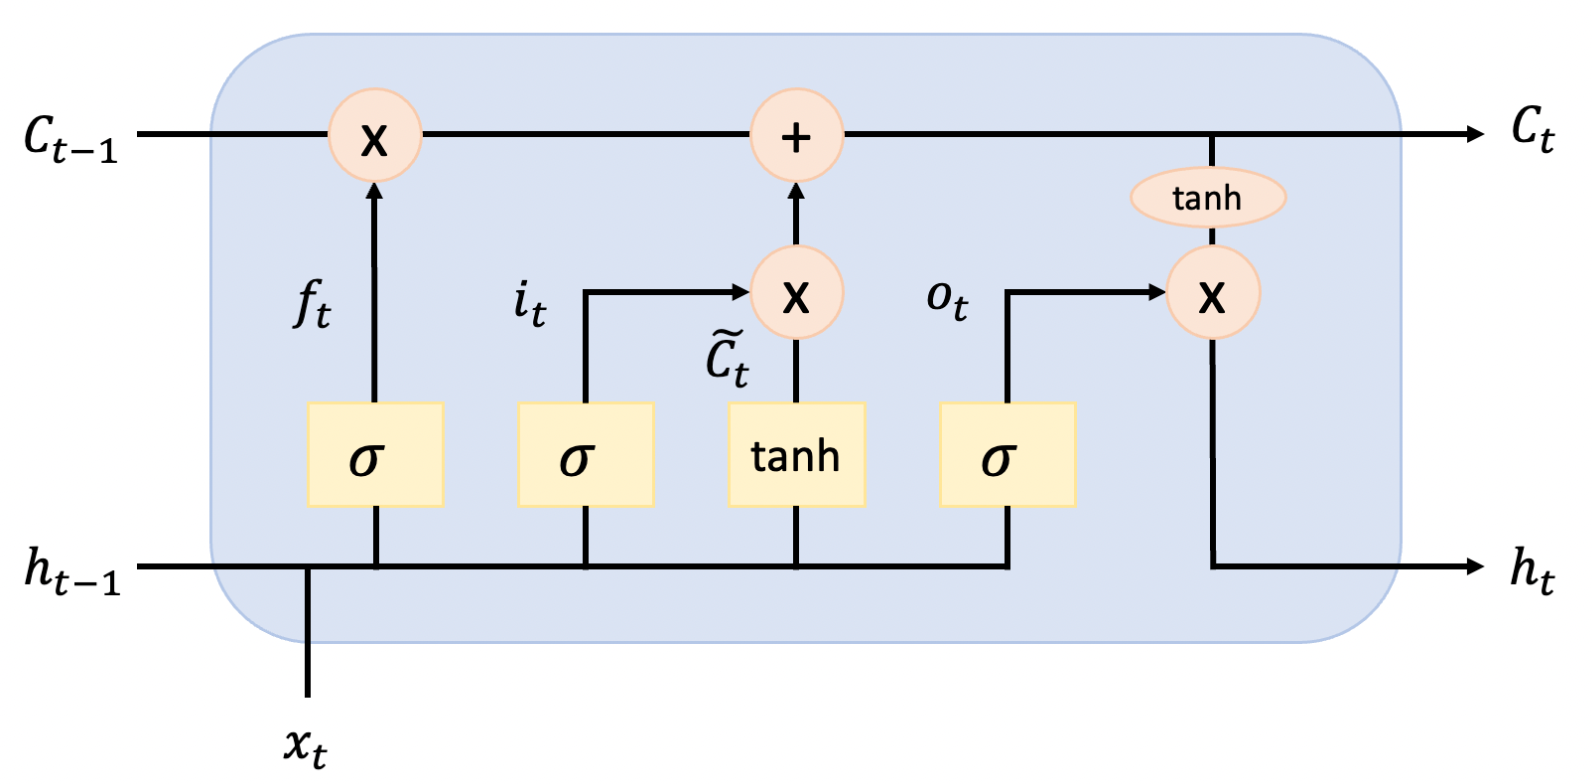
\includegraphics[width=.7\linewidth]{imported/LSTM_Cell}
    \caption{\label{fig:LSTM_Cell}长短期记忆网络单元结构示意图}
\end{figure}

LSTM(Long Short-Term Memory, 长短期记忆网络)是一种独特的循环神经网络(RNN)结构。相比于传统的RNN,
LSTM在处理序列数据上展现出了卓越的性能。
它的设计初衷是为了克服传统RNN在处理长序列时容易出现的梯度消失和梯度爆炸问题。

在动作识别中,由于同一个动作的不同阶段有不同的特征,所以给予神经网络对于过去信息的记忆能力是非常重要的,本文利用LSTM提取数据中的时间特征。

下面介绍一下LSTM的结构。LSTM网络的核心由三个关键的门结构组成:遗忘门(\(f_t\))、输入门(\(i_t\))和输出门(\(o_t\)),
这三个门结构共同工作来维护和更新一个叫做细胞状态的内部信息。

\subsubsection{遗忘门(\(f_t\))}
遗忘门的角色是确定从细胞状态中应该保留或遗弃哪些信息。数学上,其定义如下:
\begin{equation}
f_t = \sigma(W_f \cdot [h_{t-1}, x_t] + b_f)
\end{equation}

\subsubsection{输入门(\(i_t\))}
输入门确定哪些新的信息应被纳入细胞状态。它由两个部分组成:一个sigmoid层和一个tanh层。
sigmoid层决定哪些信息会被更新,而tanh层生成一个新的候选值向量,这些值可能会被纳入细胞状态中。其公式如下:
\begin{align}
i_t &= \sigma(W_i \cdot [h_{t-1}, x_t] + b_i) \\
\tilde{C}_t &= \tanh(W_C \cdot [h_{t-1}, x_t] + b_C)
\end{align}

\subsubsection{细胞状态更新}
细胞状态是LSTM的“记忆核心”,能够长时间保存信息。它受到遗忘门的影响来确定哪些信息被遗弃,同时受到输入门的指导来加入新的信息。其更新公式为:
\begin{equation}
C_t = f_t \cdot C_{t-1} + i_t \cdot \tilde{C}_t
\end{equation}

\subsubsection{输出门(\(o_t\))}
输出门决定基于细胞状态输出哪些信息。首先,我们通过一个sigmoid层确定细胞状态中哪些部分会被输出。
然后,将细胞状态通过tanh函数处理并与sigmoid门的输出相乘,这样只有选择性地输出部分信息。其公式定义如下:
\begin{align}
o_t &= \sigma(W_o \cdot [h_{t-1}, x_t] + b_o) \\
h_t &= o_t \cdot \tanh(C_t)
\end{align}

\section{粒子滤波相关技术}

\section{聚类相关技术}

\chapter{数据采集与预处理}
\section{引言}
\section{使用preamble归一化}
\section{上采样}
Decawave(Qorvo)的 DWM1000 和 NXP 的 NCJ29D5 设备的采样频率为 \(998.4 \, \text{MHz}\),对应的采样间隔为 \( \Delta \tau = 1.0016 \, \text{ns}\)。
电磁波在空气中的传播速度为 \(c = 299792458 \, \text{m/s}\),对应的波长为 \(\lambda = 0.2998 \, \text{m}\)。这个精度已经足够满足室内定位的需求。

然而,由于发送和接收设备之间的晶振并不能完全同步,导致接收到的信号的采样的相对开始时间不同步。
有一些研究者提出利用这一不同步来提高信号的采样频率,从而提高定位的精度~\cite{Ledergerber}。
也有一些研究者提出根据 IEEE 802.15.4a 规范~\cite{IEEE_Std_802.15.4a}, UWB CIR 的频谱几乎是矩形,因此可以利用 sinc 插值来提高信号的采样频率~\cite{MAMPI}。

本文借鉴了以上两种方法的思路,通过在频域中添加零来实现对信号的上采样,然后利用逆傅里叶变换(IFFT)将其转回到时域中,对结果取均值来叠加多帧的信息。下面将详细介绍上诉三种方法。

\subsection{均值滤波}
由于接收到的信号的采样的相对开始时间不同步,所以如果把λ分成多个等长的区间,每次采样只会落到其中的同一个区间,通过多次累加可以在每个区间内得到一个均值,从而提高采样率。

均值滤波算法通过以下形式的分段线性函数的系数 \( h = h_0 , h_1 , \ldots , h_{N_{\text{knots}} -1} \) 来跟踪当前测量的信道冲激响应(CIR)的均值:
\[ h(\tau ) = \frac{\tau  - \tau_i}{\Delta \tau_{\text{knots}}} h_i + \frac{\tau  - \tau_i}{\Delta \tau_{\text{knots}}} h_{i +1} \]
其中 \( i \) 满足 \( \tau_i \leq \tau < \tau_{i+1} \),并且 \( \Delta \tau_{\text{knots}} \) 是分段线性参数化的节点间的间隔。

分段线性参数化的节点 \( \tau_i \) 由以下公式给出:
\[ \tau_i = \tau_{\text{start}} + \Delta \tau_{\text{knots}} \cdot i \]
对于 \( i = \{0, \ldots , N_{\text{knots}} - 1\} \)。

节点总数 \( N_{\text{knots}} \) 由以下公式给出:
\[ N_{\text{knots}} = \frac{\tau_{\text{end}} - \tau_{\text{start}}}{\Delta \tau_{\text{knots}}} + 1 \]

分段线性函数表示CIR的均值计算复杂度低,该算法可以在每个DWM1000模块的主微控制器上运行,这对于实时处理至关重要,并且可以减少用于传输数据的空中时间。
由于其轻量化的特性,使其适用于具有有限内存和计算能力的嵌入式设备,并且可以实时执行。

\subsection{插值法}
本文主要使用了UWB的信道3与信道4。据IEEE 802.15.4a,UWB信道3的中心频率为4492.8Mhz,带宽为449.2Mhz,UWB信道4的中心频率为3993.6,带宽为1331.2Mhz。
信道3,4的频谱图像如图\ref{fig:spectrum_mask}所示,他们的频谱接近矩形,因此可以利用sinc插值来提高信号的采样频率。
\begin{figure}[htbp]
    \centering
    \includegraphics[width=.7\linewidth]{plotted/spectrum_mask}
    \caption{\label{fig:spectrum_mask}UWB信道3,4频谱}
\end{figure}

\begin{figure}[htbp]
    \centering
    \begin{subfigure}{0.33\textwidth}
        \centering
        \includegraphics[width=1.0\textwidth]{plotted/interpolation/time.png}
        \caption{\label{fig:time}原始时域图}
    \end{subfigure}%
    \begin{subfigure}{0.33\textwidth}
        \centering
        \includegraphics[width=1.0\textwidth]{plotted/interpolation/zero_time.png}
        \caption{\label{fig:zero_time}零填充后的时域图}
    \end{subfigure}
    \begin{subfigure}{0.33\textwidth}
        \centering
        \includegraphics[width=1.0\textwidth]{plotted/interpolation/sinc_time.png}
        \caption{\label{fig:sinc_time}sinc插值后的时域图}
    \end{subfigure}

    \begin{subfigure}{0.33\textwidth}
        \centering
        \includegraphics[width=1.0\textwidth]{plotted/interpolation/freq.png}
        \caption{\label{fig:freq}原始频域图}
    \end{subfigure}%
    \begin{subfigure}{0.33\textwidth}
        \centering
        \includegraphics[width=1.0\textwidth]{plotted/interpolation/zero_freq.png}
        \caption{\label{fig:zero_freq}零填充后的频域图}
    \end{subfigure}
    \begin{subfigure}{0.33\textwidth}
        \centering
        \includegraphics[width=1.0\textwidth]{plotted/interpolation/sinc_freq.png}
        \caption{\label{fig:sinc_freq}sinc插值后的频域图}
    \end{subfigure}
    \caption{sinc插值时频域图}
    \label{fig:interpolation}
\end{figure}

本文以信道3为例,介绍sinc插值的过程。

零填充:
首先,通过在原始数据样本(图\ref{fig:time})之间插入零,
对数据进行上采样。在每个原始数据样点之间插入 \( ( \text{upsample\_factor} - 1) \) 个零。
例如,如果上采样因子为4,那么在每个数据样点之间插入3个零,得到零填充后的时域图(图\ref{fig:zero_time})。
零填充的表达式如下所示:
\[
    x[n] = \{x[0], 0, 0, 0, x[1], 0, 0, 0, x[2], 0, 0, 0, \ldots\}
\]

从频域看,原始的频域图像(图\ref{fig:freq})变为零填充后的频域图像(图\ref{fig:zero_freq})。
为了使频域保持一致,需要通过在时域卷积sinc函数实现在频域的低通滤波。

构建 sinc 函数:
构建 sinc 函数以用于插值。sinc 函数是由以下公式定义的:
\[
    \text{sinc}(x) = \dfrac{\sin(\pi x)}{\pi x}
\]

在代码中,sinc 函数的参数是通过时域索引和上采样因子来调整的,以确保 sinc 函数正确对齐在零填充数据的样点上。

\[
    t = \text{np.arange}(-\text{len(zero\_padded\_data)}//2, \text{len(zero\_padded\_data)}//2) * 10^{-9}
\]
\[
    \text{sinc\_func} = \text{np.sinc}(\frac{t \cdot \text{cutoff\_frequency}}{\text{upsample\_factor} })
\]
其中zero\_padded\_data为零填充后的数据,upsample\_factor为上采样因子。
sinc函数的时频域图如\ref{fig:sinc}所示。
\begin{figure}[htbp]
    \centering
    \includegraphics[width=.7\linewidth]{plotted/interpolation/sinc.png}
    \caption{\label{fig:sinc}sinc函数时频图}
\end{figure}

卷积 (Convolution):
使用 sinc 函数对零填充的数据进行卷积,以得到插值的数据。这一步通过数学卷积操作完成,可以通过以下公式表示:
\[
    y[n] = \sum_{k=-\infty}^{\infty} x[k] \cdot \text{sinc\_func}[n - k]
\]

在代码中,这是通过 \texttt{np.convolve} 函数完成的:
\[
    \text{interpolated\_data} = \text{np.convolve}(\text{zero\_padded\_data}, \text{sinc\_func}, \text{mode}='same')
\]
从频域看,这相当于sinc函数与零填充数据的傅里叶变换的乘积,把零填充后的频域图(\ref{fig:zero_freq})转化为 sinc 插值后的频域图(\ref{fig:sinc_freq})。
从而在保证频域一致性的同时提高了时域的采样率

\subsection{fft法}
本文使用的fft法借鉴的sinc插值的原理,sinc插值是在时域上扩充信号,进行拟合,从而达到提高采样率的目的。
fft法直接在频域上进行修改,通过ifft变化得到时域的信号,从而达到提高时域采样率的目的。

\textbf{fft变换:}
首先通过fft把信号从图\ref{fig:time}变换到频域,得到图\ref{fig:freq}。
\[ X[k] = \text{FFT}\{ x[n] \} \]

\textbf{频域补零:}
然后在频域上插入零,得到图\ref{fig:sinc_freq}。这个操作相当于在时域进行上采样和sinc插值。对于4倍上采样,在频域中的每个非零点之间插入3个零,新的频域序列为:
\[ \tilde{X}[k] = \begin{cases}
X[k/4], & \text{if } k \mod 4 = 0 \\
0, & \text{otherwise}
\end{cases} \]

\textbf{ifft变换:}
然后通过ifft变化把图\ref{fig:sinc_freq}变换到时域,得到图\ref{fig:sinc_time}。也就是上采样后的信号。
\[ \tilde{x}[n] = \text{IFFT}\{ \tilde{X}[k] \} \]

相比于sinc插值,fft法的代码量更少,计算量更小,并且更加容易理解。
但是需要注意的是,fft法的频域补零的个数必须为2的整数次幂,否则会导致频域图像出现波纹,从而影响定位精度。

\section{对齐}
对齐主要由两部分组成,一个是对齐采样点,一个是对齐相位。
\begin{figure}[htbp]
    \centering
    \begin{subfigure}{0.47\textwidth}
        \centering
        \includegraphics[width=1.0\textwidth]{plotted/align/abs_cir.png}
        \caption{\label{fig:abs_cir}CIR的绝对值}
    \end{subfigure}%
    \begin{subfigure}{0.47\textwidth}
        \centering
        \includegraphics[width=1.0\textwidth]{plotted/align/real_imag_cir.png}
        \caption{\label{fig:real_imag_cir}CIR的实部和虚部}
    \end{subfigure}

    \begin{subfigure}{0.47\textwidth}
        \centering
        \includegraphics[width=1.0\textwidth]{plotted/align/abs_up_cir.png}
        \caption{\label{fig:abs_up_cir}上采样后的CIR的绝对值}
    \end{subfigure}
    \begin{subfigure}{0.47\textwidth}
        \centering
        \includegraphics[width=1.0\textwidth]{plotted/align/real_imag_up_cir.png}
        \caption{\label{fig:real_imag_up_cir}上采样后的CIR的实部和虚部}
    \end{subfigure}%

    \begin{subfigure}{0.47\textwidth}
        \centering
        \includegraphics[width=1.0\textwidth]{plotted/align/abs_time_up_cir.png}
        \caption{\label{fig:abs_time_up_cir}对齐采样点后的CIR的绝对值}
    \end{subfigure}
    \begin{subfigure}{0.47\textwidth}
        \centering
        \includegraphics[width=1.0\textwidth]{plotted/align/real_imag_time_up_cir.png}
        \caption{\label{fig:real_imag_time_up_cir}对齐采样点后的CIR的实部和虚部}
    \end{subfigure}

    \begin{subfigure}{0.47\textwidth}
        \centering
        \includegraphics[width=1.0\textwidth]{plotted/align/abs_time_phase_up_cir.png}
        \caption{\label{fig:abs_time_phase_up_cir}对齐采样点与相位后的CIR的绝对值}
    \end{subfigure}
    \begin{subfigure}{0.47\textwidth}
        \centering
        \includegraphics[width=1.0\textwidth]{plotted/align/real_imag_time_phase_up_cir.png}
        \caption{\label{fig:real_imag_time_phase_up_cir}对齐采样点与相位后的CIR的实部和虚部}
    \end{subfigure}
    \caption{对齐采样点与相位}
    \label{fig:align}
\end{figure}

\subsection{对齐采样点}
由于DWM1000和NCJ29D5收发不在一个设备上,它们的晶振并不能完全同步,导致接收到的信号的采样的相对开始时间不同步。所以本文需要对采样点进行同步,这样同一个位置的采样点对应的信号传播时间相同。

对于decawave的DWM1000模块,芯片提供first\_path,first\_path是波峰相对于第一个采集点的位置的小数部分,本文使用的数据集都选用了first\_path前4ns作为CIR的起始点。
first\_path是通过decawave内置的波峰检测算法得到的~\cite{dwm1000_user_manual},数据手册中提及算法的精度是\(\frac{1}{64}\)ns,到达了精度要求,所以对于decawave采集的数据,直接通过first\_path对齐即可。

对于NXP的NCJ29D5模块,芯片没有提供first\_path,所以需要通过其他方法获得first\_path。考虑到CIR信号稳定的特点,本文使用的对齐方法是通过correlation实现的。

\begin{figure}[htbp]
    \centering
    \begin{subfigure}{0.9\textwidth}
        \centering
        \includegraphics[width=1.0\textwidth]{plotted/first_path}
        \caption{\label{fig:first_path}不同起始点的CIR}
    \end{subfigure}%

    \centering
    \begin{subfigure}{0.9\textwidth}
        \centering
        \includegraphics[width=1.0\textwidth]{plotted/correlation}
        \caption{\label{fig:correlation}两个信号的correlation}
    \end{subfigure}%

    \caption{对齐采样点与相位}
    \label{fig:first_path_and_correlation}
\end{figure}
\subsubsection{获取first\_path}
从图\ref{fig:abs_up_cir}可以看到,不同起始点的CIR的波形都是稳定的,所以可以通过correlation计算它们的重叠程度。

本文的目标是使用相关性找到两个离散信号之间的相关程度,在重叠最多的位置相关程度最大,这个位置和信号偏移量存在固定的关系。
在图\ref{fig:first_path}中,两个信号的长度相同,分别用 \( x_1[n] \) 和 \( x_2[n] \) 在离散时间中表示。使用以下公式计算两个信号的互相关:

\[
r_{x_1, x_2}[m] = \sum_{n=-N+1}^{N-1} x_1[n] \cdot x_2[n+m]
\]

其中,\( N \) 是信号的长度。

然后扫描所得的互相关图\ref{fig:correlation},以找到最大值出现的索引,表示为 \( \texttt{peak\_index} \)。此索引对应于两个信号之间的偏移量,并在代码中如下计算:
\[
\texttt{peak\_index} = \texttt{np.argmax(correlation)}
\]
\[
m_{\text{peak}}  = (\texttt{peak\_index} - \texttt{N}) \cdot \texttt{sample\_interval}
\]
此偏移量, \( m_{\text{peak}} \),表示为对齐两个信号所需的水平移动。在这种特殊情况下,\( m_{\text{peak}} = -0.25ns \), 表示信号2左移\(0.25ns\)与信号1对齐。

对于从NCJ29D5采集的数据,本文把第一个CIR信号作为参考,把峰值点手工移动到4ns处,其它CIR样本相对于第一个CIR信号通过这种方法得到first\_path。


\subsubsection{对齐first\_path}
如图 \ref{fig:first_path} 所示,在未通过 \texttt{first\_path} 对齐的情况下,CIR 的起始点是随机的。图中蓝线被略微抬高,以便与橙线区分。

CIR 的最大值代表没有经过任何反射的直射信号,对应的距离为0。而 \texttt{first\_path} 就是这个0距离点相对于第一个采样点的位置的小数部分。不同样本在对齐前,同一采样点对应的距离是不同的。

图中蓝线的 \texttt{first\_path} 为 \(0.25\, \text{ns}\),橙线的 \texttt{first\_path} 为 \(0.5\, \text{ns}\)。为了对齐蓝线与橙线,本文舍弃蓝线前 \(0.25\, \text{ns}\) 的数据,舍弃橙线前 \(0.5\, \text{ns}\) 的数据,从而实现对齐。

由于不同的 CIR 的 \texttt{first\_path} 不同,它们舍弃的数据长度也不同。在64倍采样的情况下,舍弃的数据长度在0到63之间波动,本文会保留 \((\texttt{CIR\_LEN}-1) \times 64\) 个对齐好的采样点,这时每个样本同一采样点对应的距离相同。

具体的效果如图 \ref{fig:align} 所示。经过上采样后,CIR 由图 \ref{fig:abs_cir} 变为图 \ref{fig:abs_up_cir},此时 CIR 还未通过 \texttt{first\_path} 对齐。可以看到两条 CIR 数据虽然波形稳定,但是在水平方向有一个明显的偏差,这说明采样点没有对齐。在经过 \texttt{first\_path} 对齐后,本文得到图 \ref{fig:abs_time_up_cir},完成对于采样点的对齐。

\subsection{对齐相位}
完成采样点对齐后,如图\ref{fig:abs_time_up_cir}所示,本文可以看到复数信号的绝对值已经对齐。
然而,复数信号除了绝对值外,还包含相位信息。由于发送和接收设备之间的晶振不能完全同步,每次采样的初始相位都会有所不同。
因此,即使完成了采样点对齐,如图\ref{fig:real_imag_time_up_cir}所示的实部和虚部图也不能直接使用。

借助于CIR信号的稳定性,本文尝试对基于I/Q的CIR测量值 \( X \) 进行相位对齐,目标是最小化不同CIR数据相位的曼哈顿距离,从而最小化相位偏移的影响。
本文借鉴了\cite{IQ9452299}提出的算法,该算法的核心思想是通过小步旋转预处理的 \( X_{\text{obs}} \),
并计算旋转后的观测 \( X_{\text{rot}} \) 和参考 \( X_{\text{ref}} \) 之间的差异。
为了减少原算法的计算量,本文首先将first\_path位置的复数信号旋转到0相位,具体公式如下:
\[
X_{\text{start}} = X_{\text{obs}} \cdot e^{-j \cdot \text{angle}(X_{\text{obs}}[\text{first\_path}])}
\]
接下来,本文通过以下方式以小步旋转初始相位 \( X_{\text{start}} \):
\[
X_{\text{rot}} = X_{\text{start}} \cdot e^{j\theta}
\]
每次旋转后,本文计算参考 \( X_{\text{ref}} \) 和旋转观测 \( X_{\text{rot}} \) 之间的 \( \ell_1 \)-距离:
\[
d_{\ell_1}(X_{\text{ref}}, X_{\text{rot}}) = \sum_{n=1}^N |X_{\text{ref}}[n] - X_{\text{rot}}[n]|
\]
在预定义的相位范围\((-5^\circ,5^\circ)\)内旋转 \( X_{\text{start}} \) 后,本文找到所有计算的 \( \ell_1 \)-距离的最小值:
\[
\hat{X} = \arg\min d_{\ell_1}(X_{\text{ref}}, X_{\text{rot}})
\]
其中 \( d_{\ell_1}(X_{\text{ref}}, X_{\text{rot}}) = \{d_{\ell_1}(X_{\text{ref}}, X_{\text{rot}})\} \) 是所有计算的 \( \ell_1 \)-距离的集合。最小值 \( \hat{X} \) 表示了最佳匹配。
经过相位对齐后本文得到图\ref{fig:real_imag_time_phase_up_cir}。

\section{异常值剔除}

错误的CIR测量可能会导致后续的均值,方差积累误差,进而干扰后续模型的表现,因此本文依据以下标准排除信号。

CIR的测量主要是通过acculumator实现的,preamble accumulation count记录了accumulator收集的信号数量。
如果preamble accumulation count小于某个阈值,说明收集的信号数量太少,此时的CIR测量不可靠,应该被排除。
本文选用的阈值是64,即收集的信号数量小于64时,CIR测量不可靠。

在估计的 First\_Path 之前的CIR样本的幅度不能大于某一个特定的值,这些信号是
接收器在First\_Path到达之前收集的,反应了空间中的噪声大小,对于噪声过大的采样点本文选择排除。

测量CIR的First\_Path幅度不能与均值相差过多。当测量的First\_Path大于均值的五倍或小于两倍时,测量被拒绝。

许多原因可能导致这种错误的CIR测量,
例如DWM1000的前沿检测算法未能正确检测First\_Path位置
或当两个模块同时传输时发生数据包碰撞。


\section{方差图}
\begin{figure}[htbp]
    \centering
    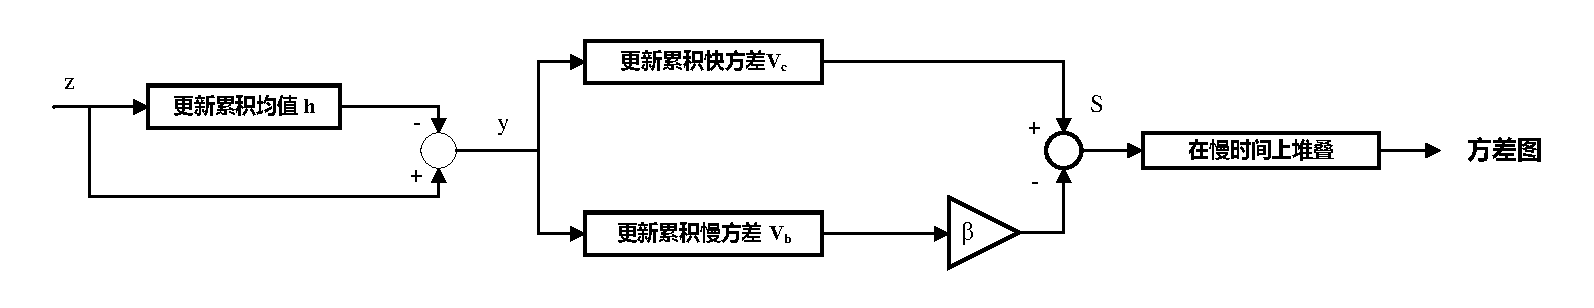
\includegraphics[width=.95\linewidth]{imported/方差图生成流程}
    \caption{\label{fig:variance_graph_pipline}方差图生成流程}
\end{figure}
当场景中出现移动对象时,它会在累积的CIR中产生具有较高方差的区域。通过分析方差图,深度学习算法可以检测到由对象的移动产生的特定模式。图\ref{fig:variance_graph_pipline}中说明了方差图生成的流程,其各个步骤如下所述。

\subsubsection{均值滤波}
由于数据已经过上采样和插值,因此均值滤波比以前\cite{Ledergerber}的方法更简单,但效果更好。本文使用累积均值来计算均值,如下所示:
\begin{equation}
    h = 0.95h + 0.05z
\end{equation}
其中,系数 \( h \) 用第一个接收到的测量值 \( z \) 初始化为 \( h = z \)。

\subsubsection{累积方差}
有了均值以后,可以进一步得到当前测量的CIR的方差度量。这一步也比以前\cite{Ledergerber}的方法更简单。本文使用两个累积均值来跟踪当前和背景方差:
\begin{align}
    V_c &= 0.9V_c + 0.1y \\
    V_b &= 0.999V_b + 0.001y
\end{align}

\subsubsection{背景减除}
通过从当前方差度量中减去背景方差度量,可以检测到CIR中具有暂时较高方差的区域,公式如下:
\begin{equation}
    S = V_c - 1.3V_b
\end{equation}
完成这三个步骤后,生成了每个样本的方差,最后本文在慢时间对样本进行堆叠,生成方差图。


\chapter{定位}
\section{引言}

\section{系统架构}

\section{数据集}

\section{概率分布图生成}

\subsection{滑动窗口}

\subsection{MARTI 加 MSR}

\subsection{神经网络}
\subsubsection{模型架构}
\begin{figure}[htbp]
    \centering
    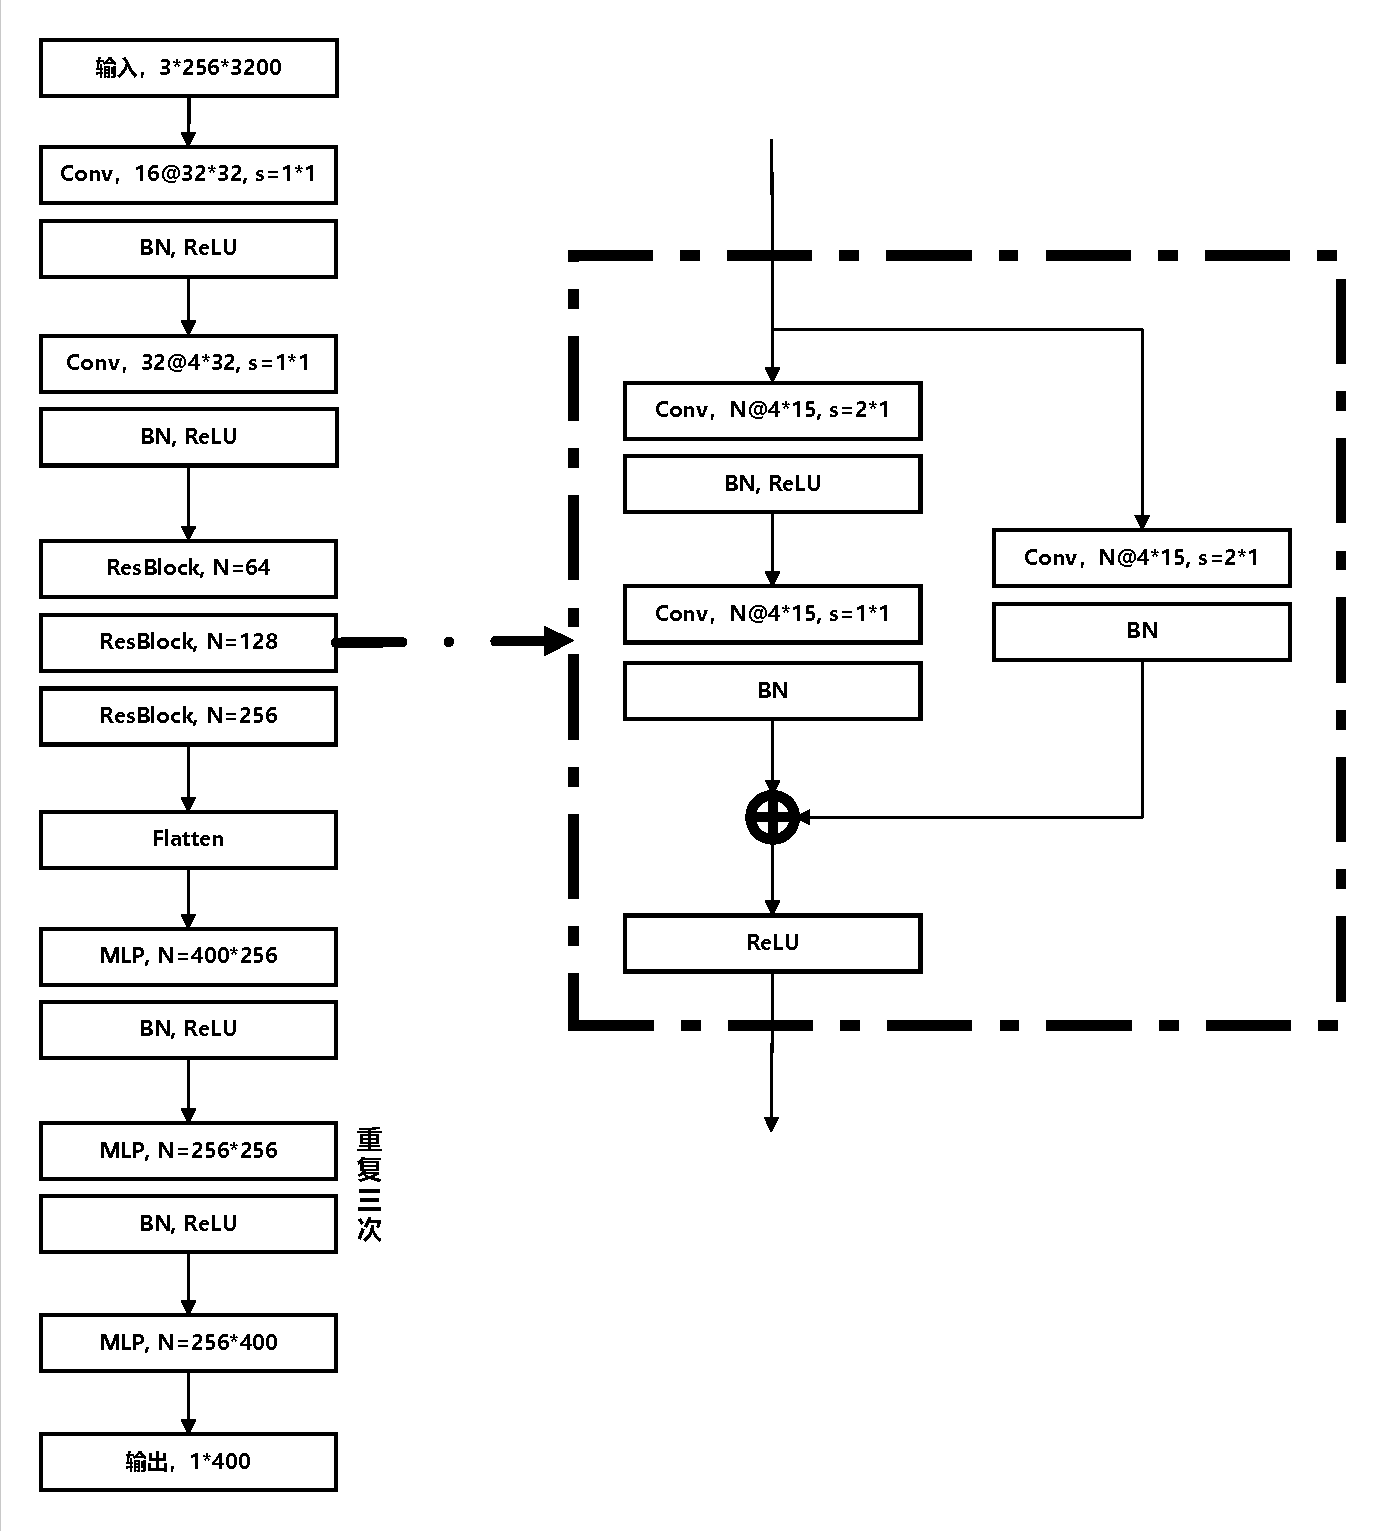
\includegraphics[width=.99\linewidth]{imported/神经网络架构}
    \caption{\label{fig:神经网络架构图}神经网络架构图}
\end{figure}
\subsubsection{推理结果}
\begin{figure}[htbp]
    \centering
    \includegraphics[width=.9\linewidth]{plotted/IPL/probability_distribution}
    \caption{\label{fig:神经网络输出概率图}神经网络输出概率图}
\end{figure}


\begin{figure}[htbp]
    \centering
    \includegraphics[width=.9\linewidth]{plotted/IPL/预测距离与真实距离}
    \caption{\label{fig:预测距离与真实距离图}预测距离与真实距离图}
\end{figure}

\section{粒子滤波与聚类}

\section{结果}


\chapter{脚踢}

\section{引言}

\section{系统架构}

\section{采集设备}


\section{数据采集与预处理}
\subsection{CAN数据转化}
控制器局域网络(Controller Area Network, CAN)是一种被广泛应用于汽车、工业自动化和航空电子等领域的网络通讯协议。
CAN总线技术自1980年代由博世(Bosch)公司开发以来,已经成为实现设备之间高效、可靠通信的重要技术。
它通过提供一种低成本、高效且可靠的通信解决方案,极大地推动了现代汽车和工业自动化系统的发展。CAN总线是车辆总线领域的国际标准(ISO 11898)\cite{Chen2009ResearchOT}。

CAN总线技术具有以下几个特点:首先,其具有高效的通信能力,能够在噪音环境中保持稳定的通信。
其次,CAN总线提供了一种简单而灵活的网络架构,可以轻松地将新设备添加到现有的网络中。
再者,通过使用错误检测和错误处理机制,CAN总线能够确保通信的可靠性和实时性。
最后,由于其开放的标准和广泛的支持,CAN总线技术得以在众多不同领域得到应用。

本文使用的超宽带数字钥匙就是通过CAN总线与车辆的电子控制单元(Electronic Control Unit, ECU)进行通讯的,
在开发过程中,本文使用电脑运行python程序,采集通过USB CAN转换器接收到的CAN数据,CAN数据里封装了脚踢检测所需要的CIR信息。

USB CAN转换器实现了CAN总线与USB总线的转换,该设备提供python库文件,可以通过已有的API函数实现CAN数据的接收和发送。
在开发阶段,本文使用电脑通过USB CAN转换器来读取CAN数据,以及运行脚踢检测的算法。开发完成以后,只需要使用嵌入式Linux设备的CAN API函数代替USB CAN设备的函数即可完成迁移。
通过该设备接收到的数据格式如下所示:

\noindent
\begin{minipage}{.5\textwidth}
    \begin{table}[H]
        \caption{\label{tab:Header}消息头格式}
        \centering
        \begin{tabular}{|l|l|}
        \hline
        Field Name & Size \\
        \hline
        Magic Number & 2 bytes \\
        \hline
        Data Count & 4 bytes \\
        \hline
        Paddings & 2 bytes \\
        \hline
        \end{tabular}
    \end{table}
\end{minipage}%
\begin{minipage}{.5\textwidth}
    \begin{table}[H]
        \caption{\label{tab:Payload}消息体格式}
        \centering
        \begin{tabular}{|l|l|}
        \hline
        Field Name & Size \\
        \hline
        Index Number & 1 byte \\
        \hline
        Payload & 7 bytes \\
        \hline
        \end{tabular}
    \end{table}
\end{minipage}
\vspace{\baselineskip} % Adds one line of vertical space

其中,消息头部分的Magic Number为85 85,Data Count记录了采集到的CIR的长度,Paddings是2个字节的无效数据。消息体部分Index Number记录了这是某个消息头下的第几个CAN包,Payload部分记录了真正的CIR数据。
每次采集到的CIR数据的长度是31个复数,每个复数由实部和虚部组成,实部占2个字节,虚部占两个字节。本文通过python程序把CAN数据包转换成其代表CIR的复数数组。

\subsection{训练集采集}
\begin{figure}[htbp]
    \centering
    \begin{subfigure}{0.45\textwidth}
        \centering
        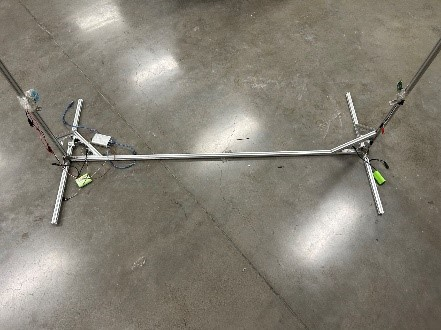
\includegraphics[width=1.0\textwidth]{imported/lab}
        \caption{\label{fig:lab}实验室布置}
    \end{subfigure}%
    \centering
    \begin{subfigure}{0.45\textwidth}
        \centering
        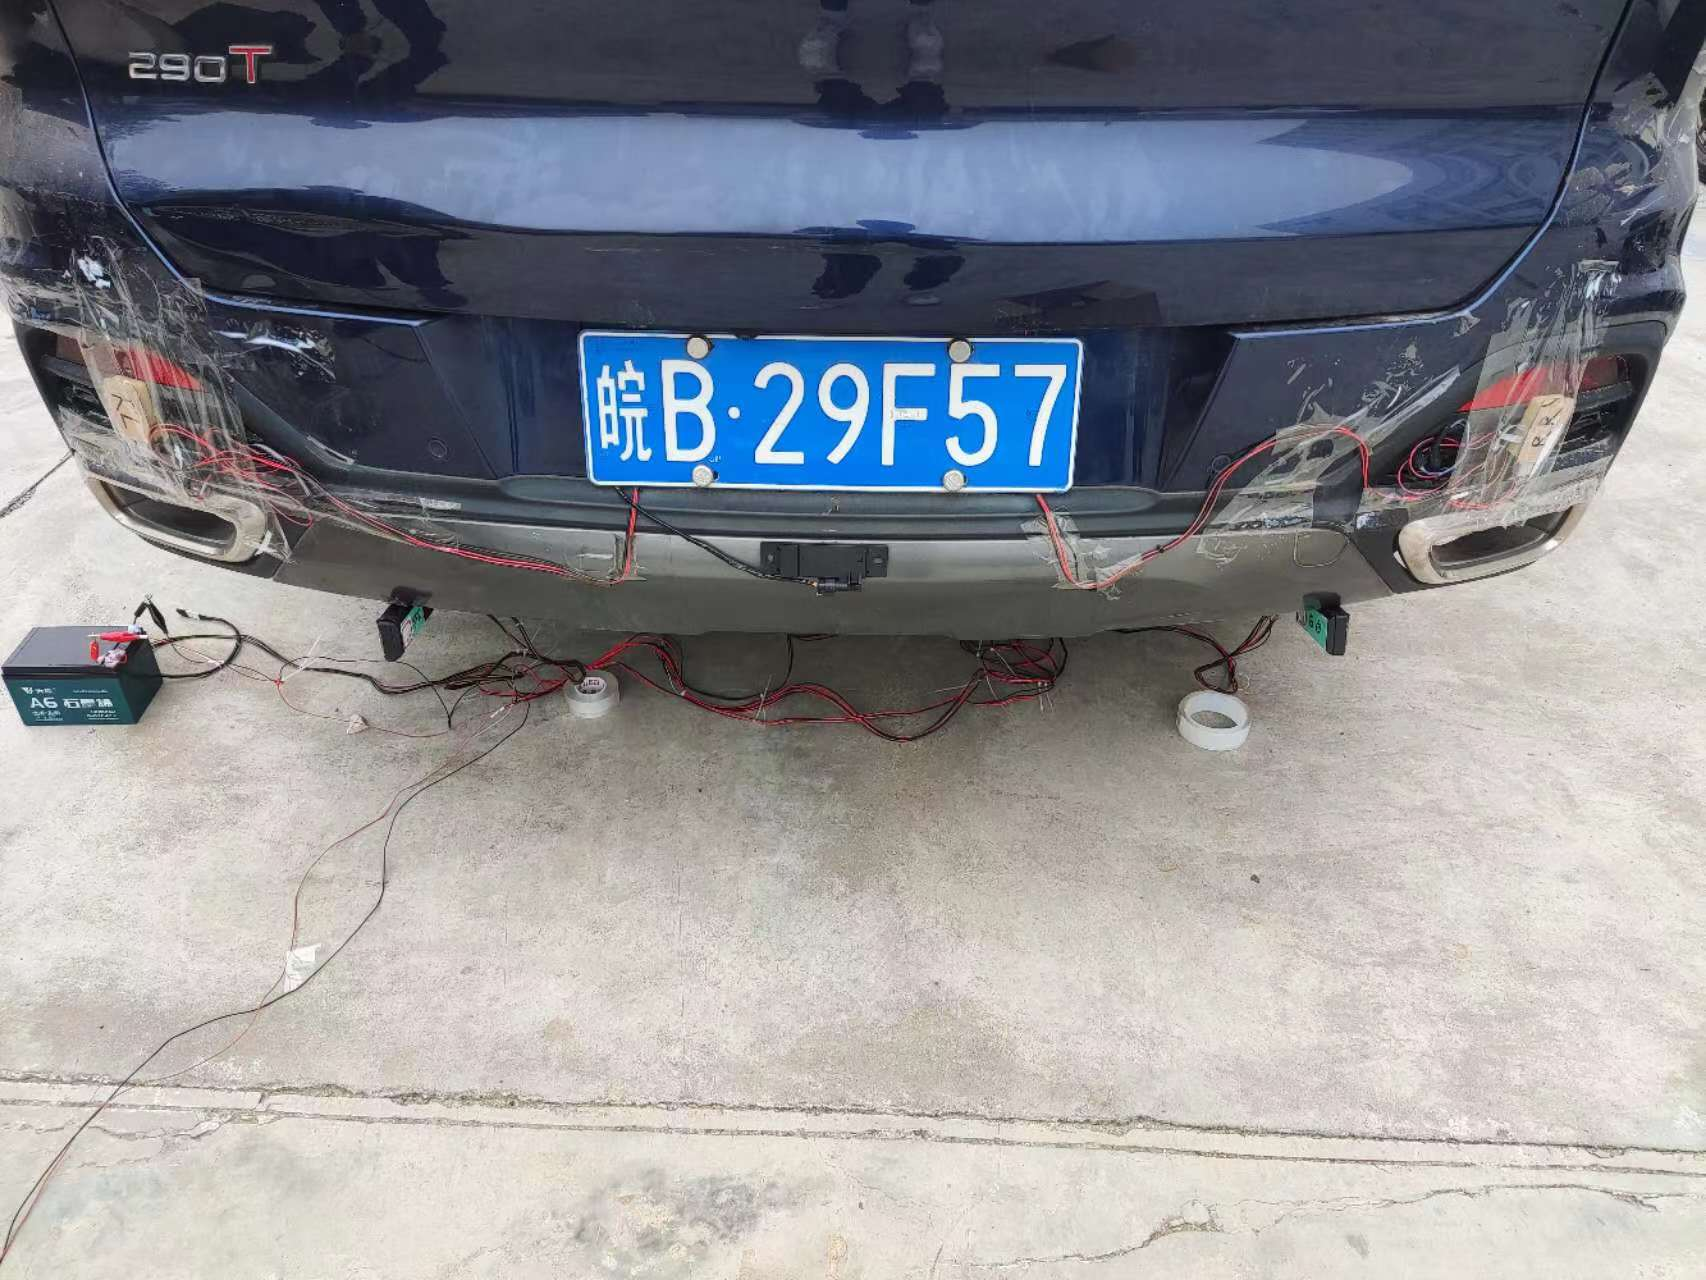
\includegraphics[width=1.0\textwidth]{imported/car}
        \caption{\label{fig:car}实车布置}
    \end{subfigure}%
    \caption{采集设备布置图}
    \label{fig:lab_car_setup}
\end{figure}
如图\ref{fig:lab_car_setup}所示,本文分别在实验室和实车上进行了实验,实验使用了两个NXP NCJ\-29D5设备,其中一个作为发送器,另一个作为接收器。
NXP NCJ29D5的频率范围为6.0 GHz至8.5 GHz。
本文的计算机持续从USB CAN中接收CAN报文并转化成CIR数据。
NXP NCJ29D5每秒生成20个CIR样本。

为了训练本文的模型,本文从七个个体收集了训练集,每个人进行大约150次水平扫腿。
每次扫腿大约持续2秒,本文通过点击鼠标记录了扫腿开始的时间,以及扫腿结束的时间,从而标注出正样本的位置。
本文手工挑选了特征强烈且清晰的数据。本文选择水平扫腿,因为它们最大化了UWB信号通道上的干扰,从而产生更清晰的信号。
为了减少误报,本文在空白背景环境中,以及人们站立、走路、跑步、跺脚或跳跃时收集负样本。本文总共收集了693个负样本,在采集负样本。

为了验证,本文收集了120个水平扫腿样本和120个其他活动的样本,每个样本有20个。本文选择了一个没有参与训练数据收集的人来记录验证数据。

在实验室中,本文使用一个铝支架将设备固定在1.6米的距离上,离地0.3米,以模拟汽车部署。本文将测试系统放在一个相对开放的区域,并使用两个12V电池供电。图7显示了实验室的设置。
在真实的汽车部署中,本文将设备放置在汽车的后备箱下方一米处,天线面向汽车的后部,以最大化信号质量并最小化对其原始数字钥匙功能的干扰。
在这两种情况下,传感器和被检测对象之间的距离均在0.4米以内。

\subsection{数据集生成}
本文首先将采集到的CAN数据转化为CIR数据。之后,CIR数据经过上采样、对齐以及异常值剔除,进入方差图生成环节。
在这个环节,我们得到了更新累积快方差 \(V_c\)、累积慢方差 \(V_b\) 以及背景减除后的方差 \(S\)。这三者 \(V_c\)、\(V_b\) 和 \(S\) 都是复数向量。
由于GPU更擅长处理实数,所以本文将它们转换为幅度向量和相位向量。这些向量在慢时间维度上进行堆叠,从而形成一个二维的时间-距离图。
其中,时间维度是慢时间,每个数据点对应0.05秒的采样间隔。
而距离维度是快时间,对应于 \( \frac{1}{64} \) 纳秒,也即0.0047米。这是基于电磁波在空气中的传播速度约为 \(2.99792458 \times 10^8 \, \text{米/秒}\)。


\section{模型设计}
\section{模型训练}
(to do: 在此处放置tensorboard产生的loss,metrics随着训练进行变化的图片)

\section{模型部署}





\chapter{呼吸}

\chapter{总结与展望}

% \chapter{关于本模板}

% 本模板根据浙江大学研究生院编写的《浙江大学研究生学位论文编写规则》~\cite{zjugradthesisrules},
% 在原有的 zjuthesis 模板~\cite{zjuthesis}基础上开发而来。

% 本模板的本科生版本\cite{zjuthesisrules}得到了浙江大学本科生院老师的支持与审核,
% 已经在本科生院网上公示。
% 但当前的研究生版本并未经过研究生院老师的审核,
% 同学们使用时要注意对照模板与要求,
% 切不可盲目使用。

% 作者本人并未编写过浙江大学研究生毕业论文,
% 所以不清楚具体要求。
% 如果有热心同学愿意帮忙,
% 可以替我联系相关老师,我会配合审核并修改代码。

% \section{Overleaf 使用注意事项}

% 如果你在Overleaf上编译本模板,请注意如下事项:

% \begin{itemize}
%     \item 删除根目录的 ``.latexmkrc'' 文件,否则编译失败且不报任何错误
%     \item 字体有版权所以本模板不能附带字体,请务必手动上传字体文件,并在各个专业模板下手动指定字体。
%           具体方法参照 GitHub 主页的说明。
%     \item 当前的Overleaf默认使用TexLive 2017进行编译,但一些伪粗体复制乱码的问题需要TexLive 2019版本来解决。
%           所以各位同学可以在Overleaf上编写论文时务必切换到TexLive 2019或更新版本来编译,以免产生查重相关问题。
%           具体说明参照 GitHub 主页。
% \end{itemize}


% \section{节标题}

% 我们可以用includegraphics来插入现有的jpg等格式的图片,
% 如\autoref{fig:zju-logo}所示。

% \begin{figure}[htbp]
%     \centering
%     \includegraphics[width=.3\linewidth]{logo/zju}
%     \caption{\label{fig:zju-logo}浙江大学LOGO}
% \end{figure}


% \subsection{小节标题}


% \par 如\autoref{tab:sample}所示,这是一张自动调节列宽的表格。

% \begin{table}[htbp]
%     \caption{\label{tab:sample}自动调节列宽的表格}
%     \begin{tabularx}{\linewidth}{c|X<{\centering}}
%         \hline
%         第一列 & 第二列 \\ \hline
%         xxx & xxx \\ \hline
%         xxx & xxx \\ \hline
%         xxx & xxx \\ \hline
%     \end{tabularx}
% \end{table}


% \par 如\autoref{equ:sample},这是一个公式

% \begin{equation}
%     \label{equ:sample}
%     A=\overbrace{(a+b+c)+\underbrace{i(d+e+f)}_{\text{虚数}}}^{\text{复数}}
% \end{equation}

% \chapter{另一章}


% \begin{figure}[htbp]
%     \centering
%     \includegraphics[width=.3\linewidth]{example-image-a}
%     \caption{\label{fig:fig-placeholder}图片占位符}
% \end{figure}

% \chapter{再一章}

% \par 如\autoref{alg:sample},这是一个算法

% \begin{algorithm}[H]
%     \begin{algorithmic} % enter the algorithmic environment
%         \REQUIRE $n \geq 0 \vee x \neq 0$
%         \ENSURE $y = x^n$
%         \STATE $y \Leftarrow 1$
%         \IF{$n < 0$}
%         \STATE $X \Leftarrow 1 / x$
%         \STATE $N \Leftarrow -n$
%         \ELSE
%         \STATE $X \Leftarrow x$
%         \STATE $N \Leftarrow n$
%         \ENDIF
%         \WHILE{$N \neq 0$}
%         \IF{$N$ is even}
%         \STATE $X \Leftarrow X \times X$
%         \STATE $N \Leftarrow N / 2$
%         \ELSE[$N$ is odd]
%         \STATE $y \Leftarrow y \times X$
%         \STATE $N \Leftarrow N - 1$
%         \ENDIF
%         \ENDWHILE
%     \end{algorithmic}
%     \caption{\label{alg:sample}算法样例}
% \end{algorithm}